%!TEX root = ReviewDraft.tex


\section{Replica wormholes}
\la{replicas} 

In this section we would like to give a flavor for the derivation of the 
formula for fine-grained entropy \cite{Lewkowycz:2013nqa,Faulkner:2013ana,Dong:2016hjy,Dong:2017xht,Penington:2019kki,Almheiri:2019qdq}. We focus on the island formula \eqref{island} for the entropy of the Hawking radiation \cite{Penington:2019kki,Almheiri:2019qdq}.

To illustrate the principle, we will consider the case when the black hole has evaporated completely and we will ignore details about the last moments of the black hole evaporation, when the interior disconnects from the exterior. For the purposes of computing the entropy,  the geometry is topologically as shown in figure \ref{BabyUniverse}(b). We want to compute the entropy of the final radiation, assuming that the black hole formed from a pure state.


  We start from the (unnormalized) initial state $|\Psi\rangle$ $-$ for example a collapsing star $-$   and evolve to the final state using the gravitational path integral which involves the semiclassical geometry of the evaporating black hole. This gives an amplitude $\langle j | \Psi\rangle$ for going from the initial state to a particular final state of radiation, $|j\rangle $ . We can now form a density matrix $\rho = |\Psi\rangle\langle \Psi|$ by computing the bra of the same state via a path integral. Its matrix elements $\rho_{ij} = \langle i |\Psi\rangle\langle \Psi|j\rangle$ are, in principle,  computed by the full gravitational path integral in figure \ref{fig:rhoLorentzianA}a. We have specified the initial and final state on the outside, but we have not been very explicit about what we do in the interior yet, and indeed, this will depend on a choice of $|i\rangle $ and $|j\rangle$.
  

\begin{figure}
\begin{center}
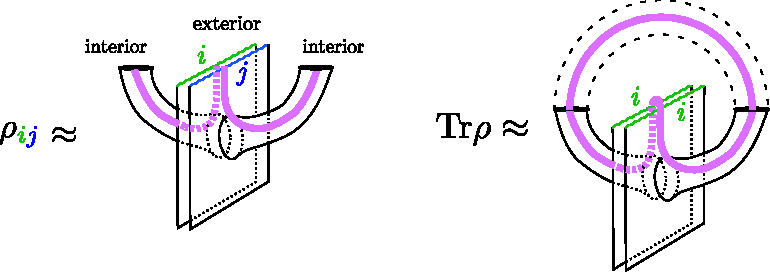
\includegraphics[scale=1]{figures/rhoLorentzianA.pdf}

~~~~~~~~~~~~(a) ~~~~~~~~~~~~~~~~~~~~~~~~~~~~~~~~~~~~~~~~~~~~~~~~~~~~~~~(b)
\end{center}
\caption{\small (a) Path integral representation of the matrix elements $\rho_{ij}$. (b) Path integral representation of $\tr \rho$. Regions with repeated indices are identified in this figure and the figures that follow. The purple line represents entanglement. \label{fig:rhoLorentzianA}}
\end{figure}

\begin{figure}
\begin{center}
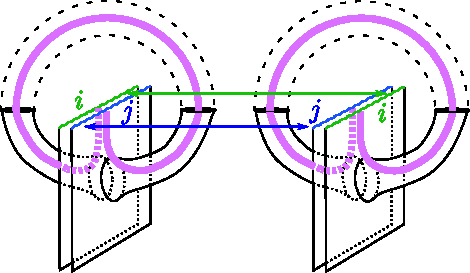
\includegraphics[scale=1]{figures/rhoLorentzianHawking.pdf}
\end{center}
\caption{\small Hawking saddle in the calculation of $\Tr[\rho^2]$. Note that following the pink line through the identifications $i \leftrightarrow i$ and $j \leftrightarrow j$ produces just one closed loop. Therefore this does not factorize into two copies of $\tr \rho$.\label{fig:rhoLorentzianHawking}}
\end{figure}

\begin{figure}
\begin{center}
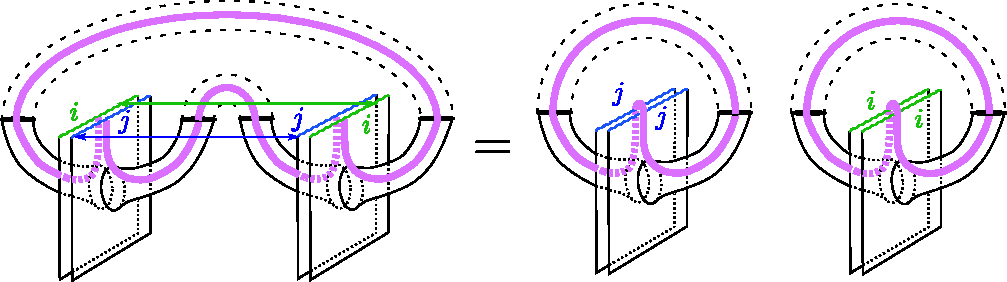
\includegraphics[scale=0.95]{figures/rhoLorentzianWormhole.pdf}
\end{center}
\caption{\small Replica wormhole saddle in the calculation of $\Tr[\rho^2]$. The black holes are joined in the interior. The second figure is just a rearrangement of the first, showing that $\Tr[\rho^2] = (\Tr[\rho])^2$. \label{fig:rhoLorentzianWormhole}}
\end{figure}


  
 The trace of the density matrix, 
  \be
\tr \rho = \sum_{i} \langle i|\Psi\rangle\langle \Psi|i\rangle \ , 
  \ee
  is computing by identifying the final state of the bra and the ket and summing over them. This gives
  the geometry in figure \ref{fig:rhoLorentzianA}b. (For those who know, this is really an in-in Schwinger-Keldysh diagram.)
   We want to diagnose whether the final state has zero entropy or not. 
  For that purpose, we compute the so-called ``purity'' of the state, defined as $\tr[\rho^2]$. If $\rho$ is an unnormalized {\it pure state} density matrix then $\tr[\rho^2] = ( \tr[\rho])^2$, while if it has a large entropy we expect $ \tr[\rho^2 ]   \ll ( \tr[\rho])^2 $.
  
  
  We can compute $\tr[\rho^2]$ via a path integral argument by connecting the exterior regions as shown in figures \ref{fig:rhoLorentzianHawking} and \ref{fig:rhoLorentzianWormhole}. A key point is that, in gravity, we should typically consider a sum over all possible topologies.\footnote{ This sum is very clearly required in some examples of AdS/CFT to match CFT properties
  \cite{Witten:1998zw}.}   This implies that 
   we should sum over different ways of   connecting the interiors.  Figures \ref{fig:rhoLorentzianHawking} and  \ref{fig:rhoLorentzianWormhole} show two different ways of connecting the interior. The first diagram, 
   figure \ref{fig:rhoLorentzianHawking}, gives the Hawking answer with its large entropy, so that 
  \be \tr[\rho^2 ]|_{\rm Hawking~saddle}  \ll ( \tr[\rho])^2 \la{HSad} \ .
  \ee 
    The second diagram, figure \ref{fig:rhoLorentzianWormhole}, which is called a replica wormhole, gives 
   \be \la{WSad}
   Tr[\rho^2]|_{\rm Wormhole~saddle}  = (\tr[\rho])^2
   \ee
    and therefore has zero entropy. The contribution of the replica wormhole is larger and it therefore dominates over the Hawking saddle \nref{HSad}.      We conclude that the leading order contribution gives the expected answer from unitarity, \nref{WSad}. 

The contribution in figure \ref{fig:rhoLorentzianHawking} is still present and one could worry that it would spoil the agreement. We will not worry about exponentially small contributions,  hoping that this (small) problem will be fixed in the future. 
   
   This calculation is very similar to the Gibbons-Hawking calculation of the black hole entropy reviewed in section \ref{ss:gibbonshawking}. The Hawking saddle and the replica wormhole saddle in Euclidean signature are drawn in fig. \ref{fig:euclidean-wormholes}. In the Hawking calculation we have two copies of the cigar geometry, while in the replica wormhole the black holes are joined through the interior.  These pictures are schematic because the actual replica wormhole for an evaporating black hole is a complex saddlepoint geometry.
   
\begin{figure}
\begin{center}
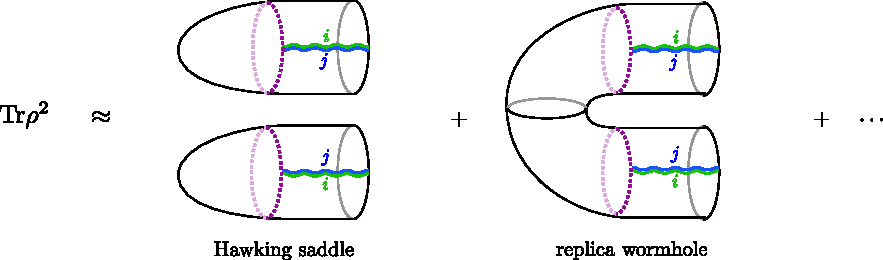
\includegraphics[scale=1]{figures/euclidean-wormholes.pdf}
\end{center}
\caption{\small Euclidean replica wormholes for computing the purity of the radiation outside the cutoff surface. The dots denote other possible topologies, which are generally subdominant. \label{fig:euclidean-wormholes}}
\end{figure}     
   

   
   The calculation of the von Neumann entropy is a bit more complicated, but the spirit is the same. We use the replica method. That is, to compute the entropy,  we consider $n$ copies of the system and compute $\tr[\rho^n]$, where $\rho$ is the density matrix of either the black hole or the radiation. We then analytically continue in $n$ and compute the entropy,
\be
S = (1-n \p_n) \log\tr [\rho^n]_{n=1} \ .
\ee
For $n \neq 1$, the black hole interior can be connected in various ways among the $n$ copies. If they are disconnected we get the usual Hawking answer for the entropy, and if they are completely connected we get the answer from the new quantum extremal surface, after continuing to $n \to 1$. The minimum of the two dominates the path integral and gives the unitary Page curve, see \cite{Penington:2019kki,Almheiri:2019qdq} (see also \cite{Marolf:2020xie,Hartman:2020swn}).



